\documentclass{beamer} 

% Michael Maier, 2013.
% CC-BY-SA

\usepackage[utf8]{inputenc}
\usepackage[ngerman]{babel}

\title{OpenStreetMap - Die freie Wiki-Weltkarte} 
\author{Michael Maier \textless Michael.Maier@student.tugraz.at\textgreater} 
\date{8. April 2014} 

\usetheme{Antibes}

\hypersetup{colorlinks=true,urlcolor=blue,linkcolor=white}

%\usebackgroundtemplatei{
%
\includegraphics[width=\paperwidth,
%height=0.8\paperheight]{mag_map.png}
%}

\begin{document}

%\maketitle

\begin{frame} 


\begin{figure}
  \centering
  
\includegraphics[width=.5\textwidth]{mag_map.png}
\end{figure}

\begin{center}
\Huge{OpenStreetMap\\}
\end{center}

\begin{center}
\Large{\emph{Die freie Wiki-Weltkarte}}
\end{center}

\end{frame}


\begin{frame}{Vorstellung}

  \begin{itemize}
    \item Michael Maier \textless \href{mailto:Michael.Maier@student.tugraz.at}{Michael.Maier@student.tugraz.at}\textgreater
    \item Student an der TU Graz (Telematik)
\vspace{0.3cm}
    \item Linux-User (Debian/grml) seit 2004
    \item Organisiere Grazer Linuxtage seit 2011 mit
    \item OpenStreetMap als Hobby seit Juli 2010
    \item Leite den Grazer OSM-Stammtisch seit Mai 2011
\vspace{0.3cm}
    \item Vorträge und Workshops zum Thema OSM seit 2012
    \item Freiberuflich OSM-Aufträge und Consulting
    \begin{itemize}
      \item OSM-username: \emph{\href{http://www.openstreetmap.org/user/species}{species}}
      \item Github-Account: \emph{\href{https://github.com/species}{species}}
      \item Twitter-Account: \emph{\href{https://twitter.com/osmgraz}{@osmgraz}}
    \end{itemize}
  \end{itemize}
\end{frame}


\section{Einleitung}

\begin{frame}{Was ist OpenStreetMap}

\begin{itemize}
  \item OpenStreetMap (OSM) ist eine freie Weltkarte nach dem Wiki-Prinzip "`Wikipedia der Karten"'
\pause
  \item Entsteht aus der Arbeit von \textgreater 1,5\,M Hobbykartografen "`\emph{Mapper}"'
\end{itemize}

 \begin{center}
 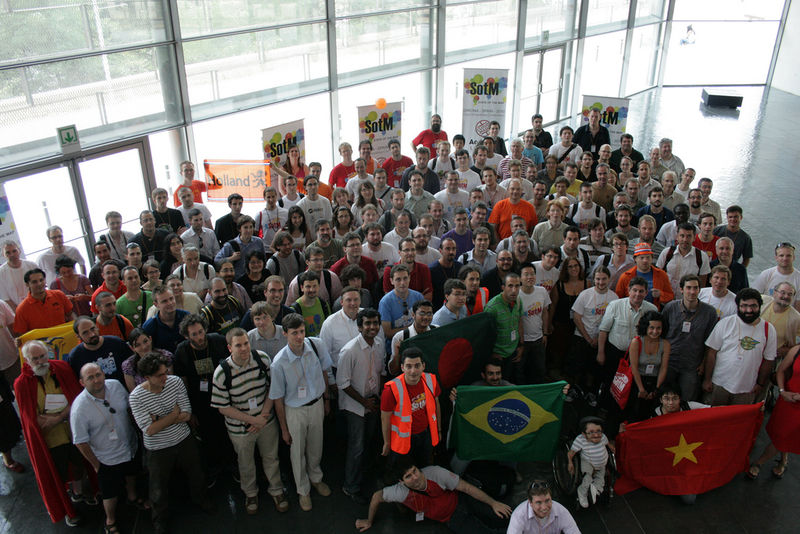
\includegraphics[width=5.5cm]{sotm.jpg}
 \end{center}

\end{frame}

\subsection{Warum OpenStreetMap?}

\begin{frame}{Warum OpenStreetMap?}

\hspace{0.5cm}Es beginnt 2004 mit einer Geschichte:
  \vspace{0.3cm}

Ein Student ärgert sich, dass es in UK keine freien Geodaten gibt.
  \vspace{0.3cm}

\parbox{9.5cm}{Die Daten auf streetmap.co.uk wurden mit Steuergeldern erstellt, man kann die Rohdaten jedoch nicht frei verwenden.}
\hfill
\raisebox{\dimexpr-\height+\baselineskip}{
\includegraphics[height=1cm]{traurig.png}}

  \vspace{0.6cm}
\pause

Warum muss man für etwas, was bereits von der Allgemeinheit mit Steuergeld bezahlt wurde, nocheinmal bezahlen?
  \vspace{0.3cm}

\parbox{9.1cm}{Und darf es selbst dann nicht frei Nutzen? \\Doppelbesteuerung ist zumindest bei uns verboten?}
\hfill
\raisebox{\dimexpr-\height+\baselineskip}{
\includegraphics[height=1cm]{grantig.png}}

\pause

 \parbox{7.5cm}{\vspace{0.4cm}\hspace{0.5cm}$\Longrightarrow$ \hspace{0.5cm}Er gründet OpenStreetMap!}
\raisebox{\dimexpr-\height+\baselineskip}{
\includegraphics[height=1.2cm]{laugh.png}}

\end{frame}


\begin{frame}{Wir brauchen freie Karten!}
Vorhandene Geodaten 
\begin{itemize}
  \item	für kommerzielle Nutzung zu teuer
  \item	wenn es sie denn gibt - zB Haiti
  \item	gratis nur für Lehre und Forschung
\end{itemize}

\pause
\vspace{2mm}
Karten kommerzieller Anbieter nur sehr restriktiv nutzbar
\begin{itemize}
  \item Restriktive Lizenzen - only Free as in Beer
  \item Offline-Nutzung oft nicht erlaubt - Roaming!
  \item Absichtliche Fehler, Änderungen/Richtigstellungen?
  \pause
  \item Beispiel Bing TOS: Durch die Nutzung schließen sie einen rechtsgültigen Vertrag mit Microsoft - Dürfen unmündige Personen (unter 18?) Bing Maps überhaupt nutzen?
  \item Kosten! Google verlangt z.B. ab 25K API-Zugriffen/Tag!
\end{itemize}

\end{frame}


\subsection{Geschichte}

{
 \usebackgroundtemplate{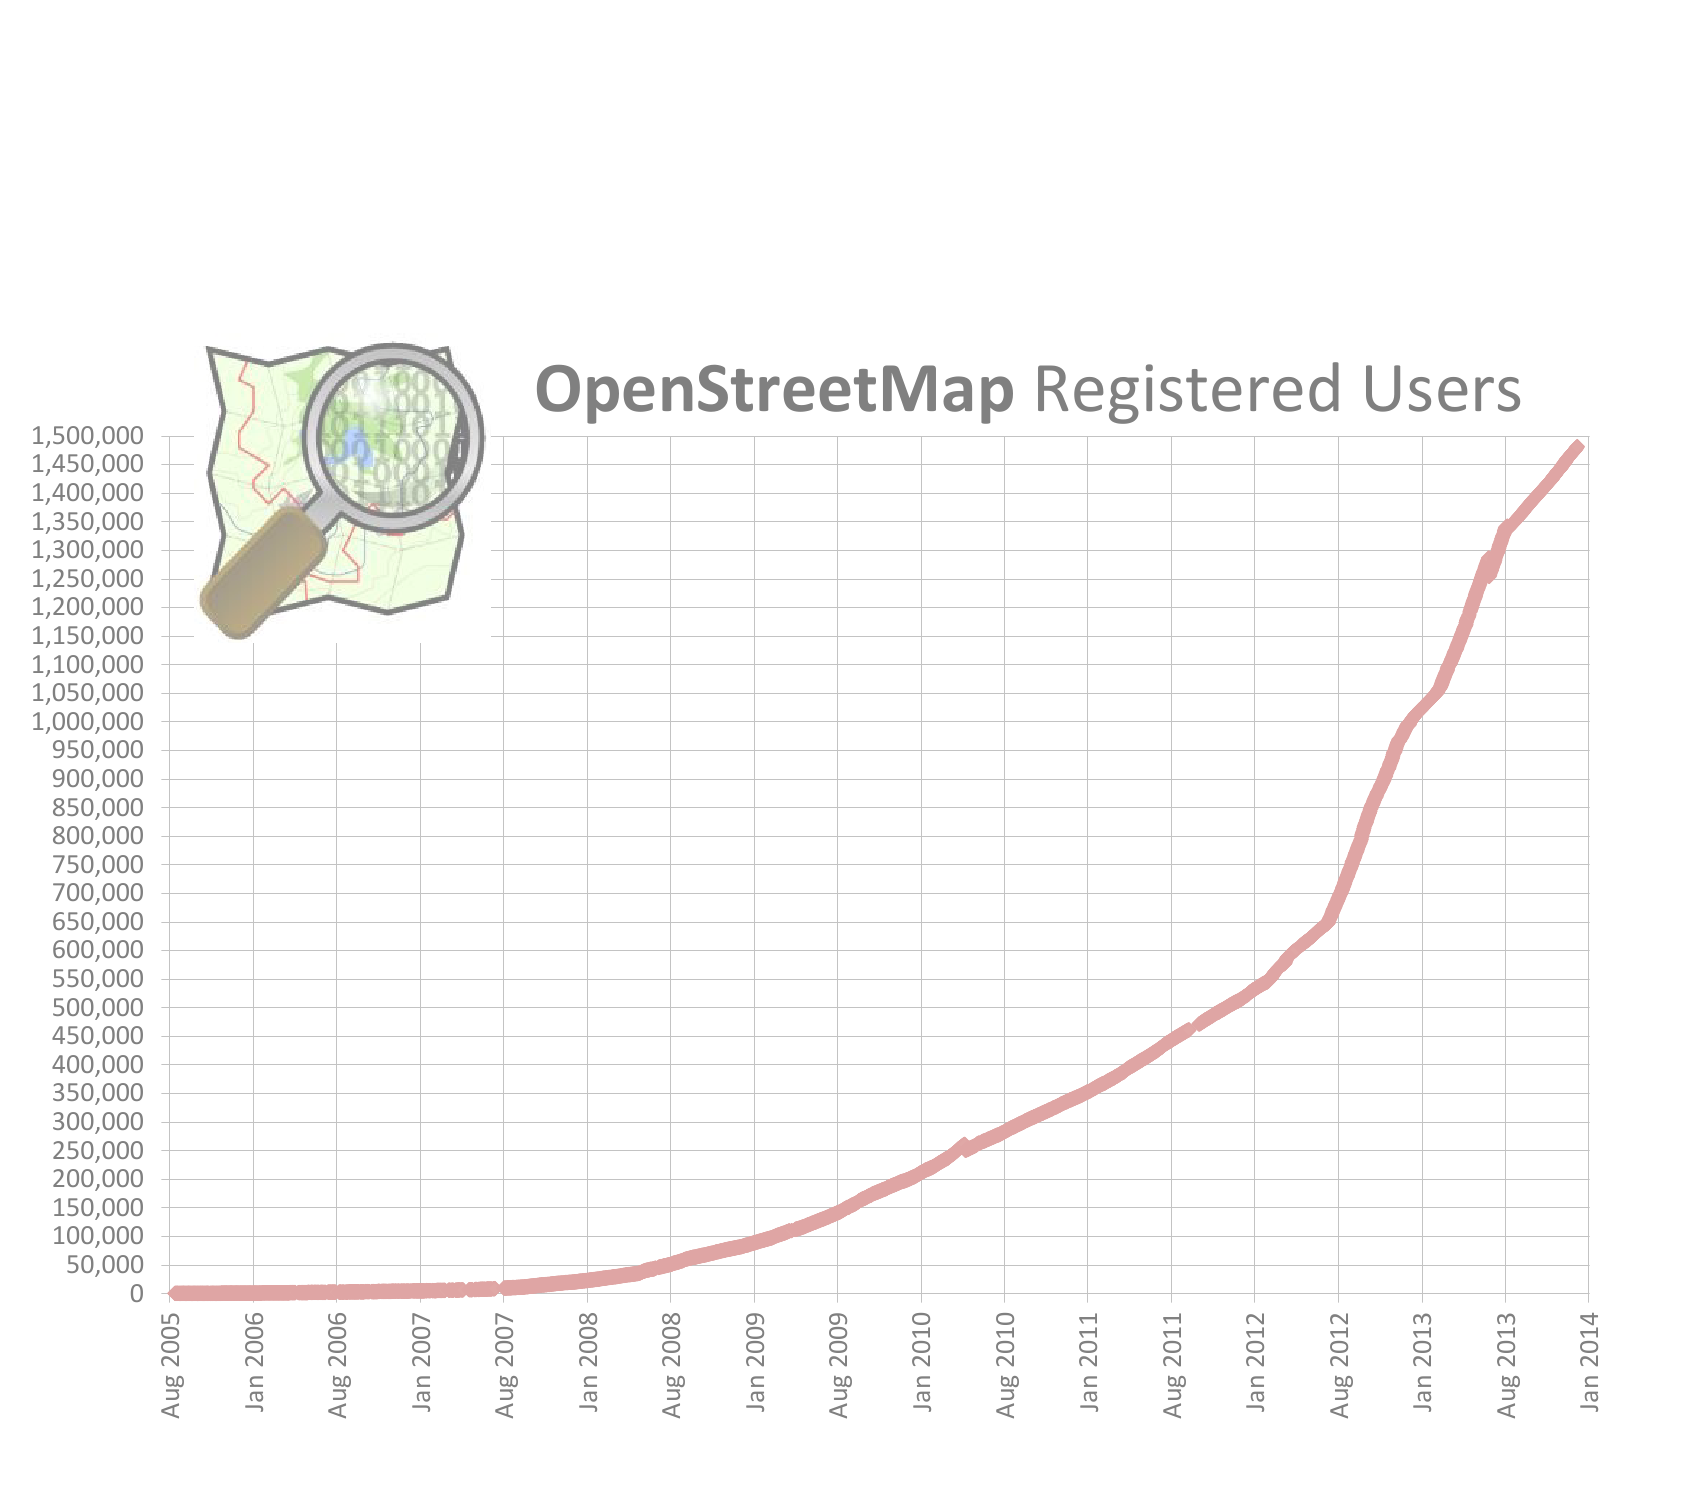
\includegraphics[height=10cm]{Osmdbstats2_users.png}}

% stats from http://www.openstreetmap.org/stats/data_stats.html

\begin{frame}{Geschichte von OpenStreetMap}
  \vspace{0.6cm}
\begin{itemize}
  \item Start des Projekts im August 2004 durch \emph{Steve Coast}
  \item Dezember 2006 - Yahoo erlaubt abzeichnen
  \item Juli 2007 - Erste Konferenz, "`State Of The Map"'
  \item August 2007 - 10.000 Registrierte Benutzer
  \item März 2009 - 100.000 Registrierte Benutzer
  \item Januar 2010 - Haiti--Projekt
  \item November 2010 - Bing erlaubt abzeichnen
  \item Juli 2011 - Erste "`State Of The Map Europe"' in Wien
  \item Januar 2013 - 1.000.000 Registrierte Benutzer
  \item Heute - 1.582.248 Registrierte Benutzer
\end{itemize}

\end{frame}
}


\subsection{Hintergrund}

\begin{frame}{Wer steht hinter OpenStreetMap}

  \begin{itemize}
    \item OpenStreetMap Foundation (Server, Rechtliche Vertretung)
      \pause
    \item Mapper ($\sim$20.000 aktiv), meist ohne Geo-Hintergrund
    \begin{itemize}
      \item Jährliche Konferenz - "`State of the Map"', heuer: Buenos Aires
    \end{itemize}
      \pause
    \item Universitäten
    \begin{itemize}
      \item Bakk-, Master- und Doktorarbeiten mit OSM
      \item Server-Hosting
    \end{itemize}
      \pause
    \item Organisationen, die Daten sponsern
    \begin{itemize}
      \item Firmen wie Yahoo/Bing, die Luftbilder zur Verfügung stellen
      \item Regierungen mit besseren Open-Data-Gesetzen als Österreich
  % BSP TIGER, USA
  % Dänemark, Hausnummern
  % Frankreich,Tschechien: Kataster
    \end{itemize}
      \pause
    \item Firmen die mit OSM arbeiten, z.B.:
    \begin{itemize}
      \item Geofabrik (de)
      \item MapBox (us)
      \item BikeCityGuide (Graz)
    \end{itemize}
  \end{itemize}

\end{frame}

\section{OpenStreetMap-Basics}

\begin{frame}{Woher kommen unsere Daten?}

\begin{itemize}
  \item Ursprünglich: GPS-Tracks
  \item Freiwillige tragen ihr Wissen bei: Jeder weiß viel über seine Umgebung:
        \begin{itemize}
          \item Hausnummern, Straßennamen,
          \item Restaurants, Bars, POIs, \dots
  \end{itemize}
  \pause
  \item Bei Mapping-Parties werden \\ gezielt Gebiete verbessert
\end{itemize}

  \vspace{0.4cm}
 99\% Handarbeit!

  \vspace*{-2.9cm}
 \hfill 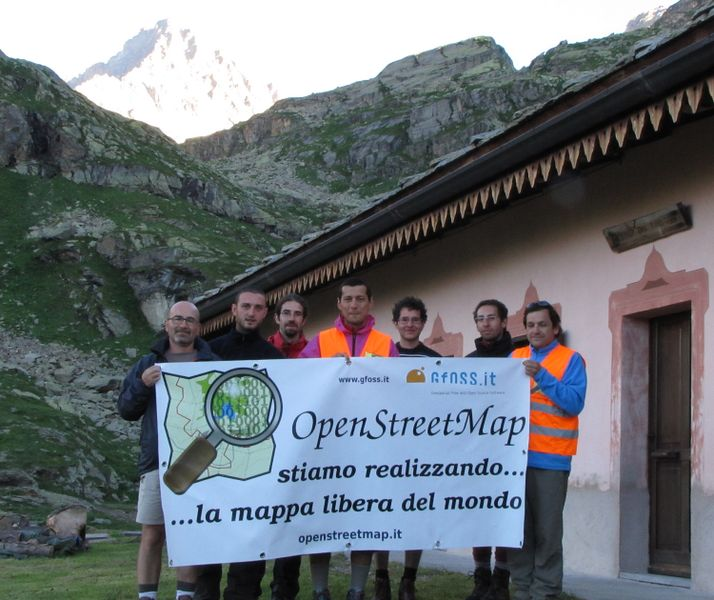
\includegraphics[width=4.2cm]{alps_mp.jpg}


  \pause
\begin{itemize}
  \item Hin und wieder Importe aus Open Government Data
  \begin{itemize}
    \item USA, TIGER Data (2008)
    \item Dänemark, Hausnummern (laufend synchronisiert)
    \item Wien, Baumkataster
  \end{itemize}
\end{itemize}

\end{frame}

\begin{frame}{Qualitätssicherung}
Ähnlich Wikipedia, jeder darf alles ändern!
  \begin{columns}[c]
    \begin{column}[T]{.35\textwidth}
      \vspace{1cm}
      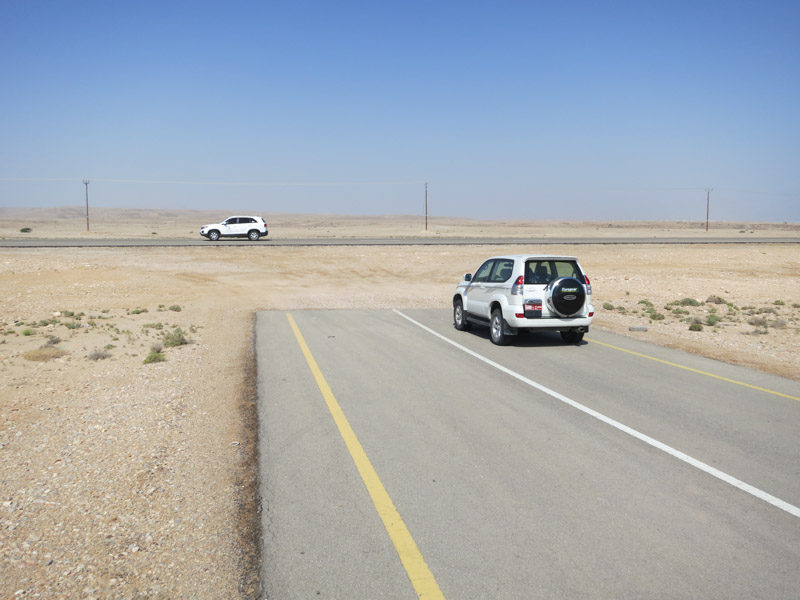
\includegraphics[width=4.5cm]{unconnected.jpg} \\
      {\TINY CC-BY \url{http://www.bodenseepeter.de}}
    \end{column}
    \pause
    \begin{column}[T]{.7\textwidth}
      \begin{itemize}
        \item Jedoch konfliktfreier als bei Wikipedia:
        \begin{itemize}
          \item Es gibt in OSM nur "`Ground Truth"'
          \item Eintrittsschwelle ist höher (keine Anonymous edits)
        \end{itemize}
        \item Erfahrene Mapper kontrollieren ihr Gebiet mittels RSS-Feed
        \pause
        \item Eingebautes Social Network: Jeder Mapper kann persönlich kontaktiert werden
        \begin{itemize}
          \item Diskussion über die Mailingliste
        \end{itemize}
        \pause
        \item Automatische Qualitätssicherungs-Tools
        \begin{itemize}
          \item \href{http://keepright.ipax.at/report\_map.php?zoom=14&lat=48.20808&lon=16.37221}{keepright.ipax.at}
        \end{itemize}
      \end{itemize}

    \end{column}
  \end{columns}

\end{frame}


\begin{frame}{Lizenz}

Die Daten stehen unter der Open Database Licence - Entspricht etwa Creative Commons - Attribution - Sharealike für Daten.
\begin{itemize}
  \item Jeder darf die Daten, auch kommerziell verwenden
  \item Quelle: "`OpenStreetMap and Contributors, ODbL"' muß angegeben werden.
\end{itemize}

 \begin{center}
 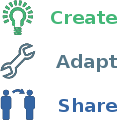
\includegraphics[width=1cm]{ODbL.png}
 \hspace{2cm}
 
\includegraphics[width=1.5cm]{cc-by-sa.pdf}
 \end{center}

\pause
Die Web-Karten auf \href{http://osm.org}{openstreetmap.org} sind CC-BY-SA.
\begin{itemize}
  \item Beachte Tile Usage Policy!
\end{itemize}

\end{frame}

\subsection{Technisches}

\begin{frame}{Freie Software für freie Daten}

Nicht nur die Daten sind frei, sondern auch die Software um die Daten zu verwalten, generieren und verwenden.

\vspace{0.6cm}

Es wird zu 100\% Freie Software verwendet. Beispiel osm.org:
\begin{itemize}
  \item Hauptdatenbank: (PostgreSQL/PostGIS)
  \item Renderstack: Mapnik/Tirex
  \item Webserver: Apache/mod\_tile
  \item Webfrontend: Leaflet
  \item Web-Backend: Basiert auf Ruby on Rails
  \item Doku-Portal: Mediawiki
\end{itemize}


  \vspace*{-3cm}
 \hfill 
\includegraphics[width=3cm]{tux.png}


\pause

Z.B verwendet \href{http://openaviationmap.org/}{openaviationmap.org} dieselben Technologien.

\end{frame}

\begin{frame}{Serverinfrastruktur}
Es gibt eine zentrale Datenbank (PostgreSQL/PostGIS) für Schreibzugriffe (in GB).\\
\pause
Diese wird weltweit gespiegelt für Lesezugriffe mit unterschiedlichen Methoden:

\begin{itemize}
  \item API-Lesezugriffe über mehrere Spiegel-Server lastverteilt
  \item Rendering-Server nutzen eine lokale, minütlich aktualisierte Datenbank
  \begin{itemize}
    \item Tileserver über GeoDNS weltweit verteilt (meist von Sponsoren)
  \end{itemize}
  \item Extrakte zum Download siehe \href{http://wiki.osm.org/Planet}{wiki.osm.org/Planet}
  \item Für räumliche SQL-Abfragen: Overpass API, zB alle italienischen Restaurants in Wien
\end{itemize}

\end{frame}



\section{Was kann ich mit OpenStreetMap machen?}

% was kann ich mit osm machen?
% Karte ansehen
% * oder in Webseiten einbinden
% * Stile
% Suche
% Routing, auch Fahrrad oder Rollstuhl
% Apps, Vorteil: Offline!
% Daten runterladen, um Analysen zu machen
% Spezialkarten machen
% * Cycle Map / hike-map
% * Seamap
% * lokalisierte karten
% darstellung von POIs
% * screenie opengastromap.de
% * overpass-turbo

\begin{frame}{OpenStreetMap.org}

	Suchfunktion:

	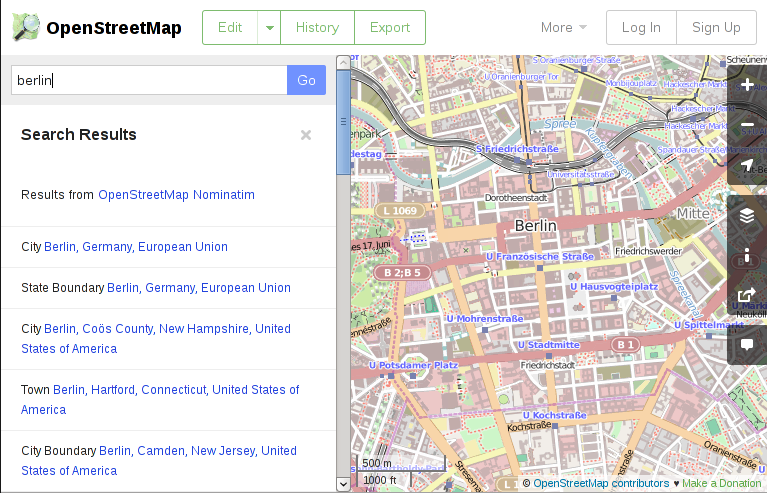
\includegraphics[width=10cm]{osm-org.png}

\end{frame}

\begin{frame}{in Webseiten einbinden}

	z.B. \url{www.linuxtage.at}

	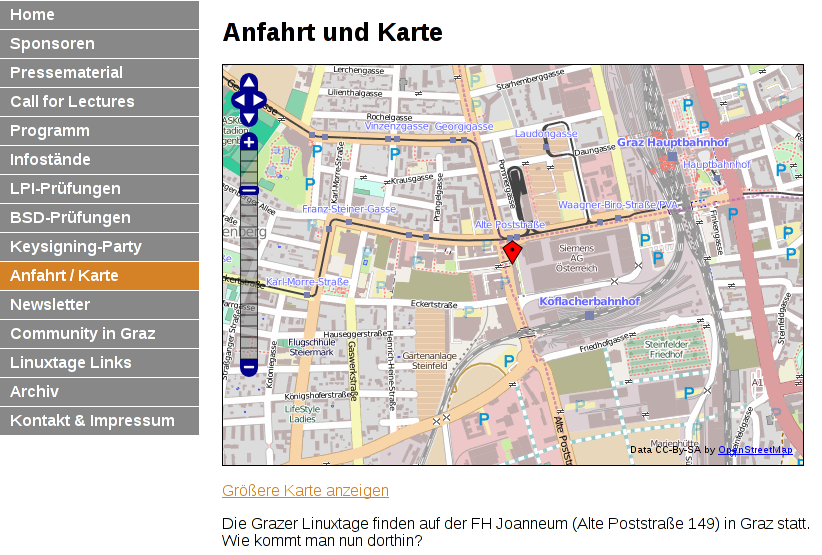
\includegraphics[width=10cm]{glt.png}

\end{frame}

\hypersetup{urlcolor=cyan}
\begin{frame}{Routing: z.B. für Rollstühle \hfill\href{http://rollstuhlrouting.de}{rollstuhlrouting.de}}

	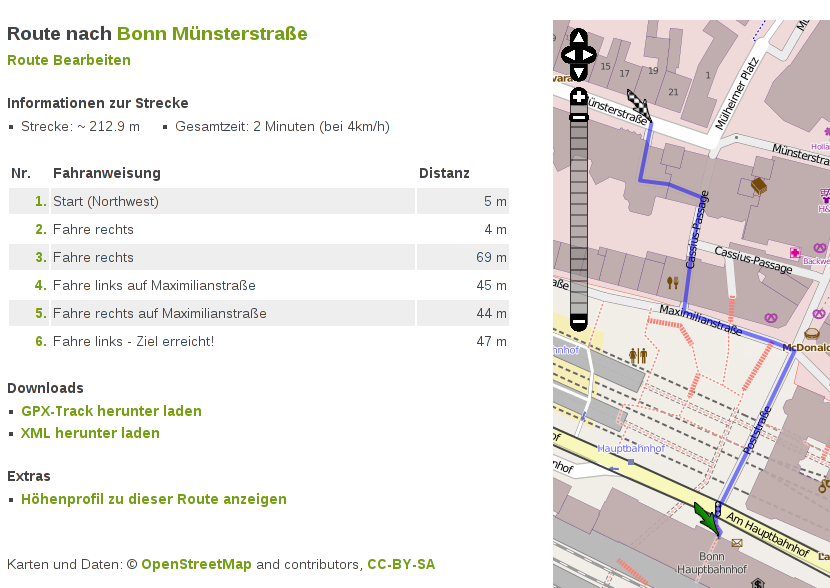
\includegraphics[width=10cm]{wheelchair-router.png}

\end{frame}
\hypersetup{urlcolor=blue}


\begin{frame}{Mobil Nutzen}
	Apps:
 
 \begin{itemize}
   \item  Android ( \textgreater 70) \url{http://wiki.osm.org/Android}
   \item  iPhone ( \textgreater 60 )  \url{http://wiki.osm.org/Apple\_iOS}
   \item  Blackberry ( 8 ) \url{http://wiki.osm.org/BlackBerry\_OS}
 \end{itemize}
 
 \begin{center}
 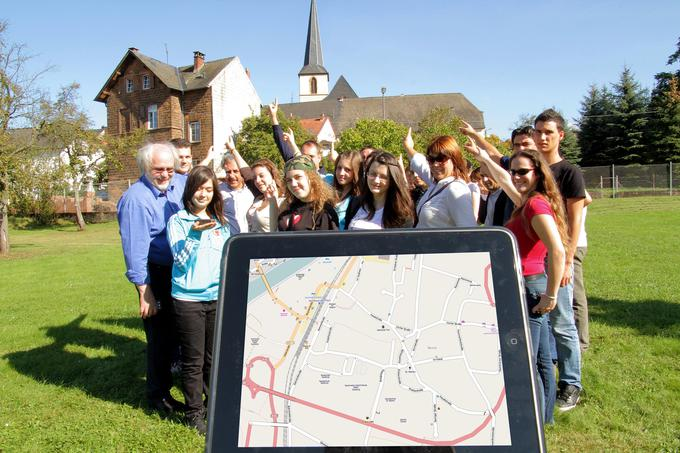
\includegraphics[width=5cm]{tablet.jpg}
 \end{center}

 Natürlich auch auf Navis, am OSM-freundlichsten sind Garmin: \href{http://wiki.osm.org/Garmin}{wiki.osm.org/Garmin}!

\end{frame}

\begin{frame}{Spezialkarten: z.B. OpenSeaMap}

 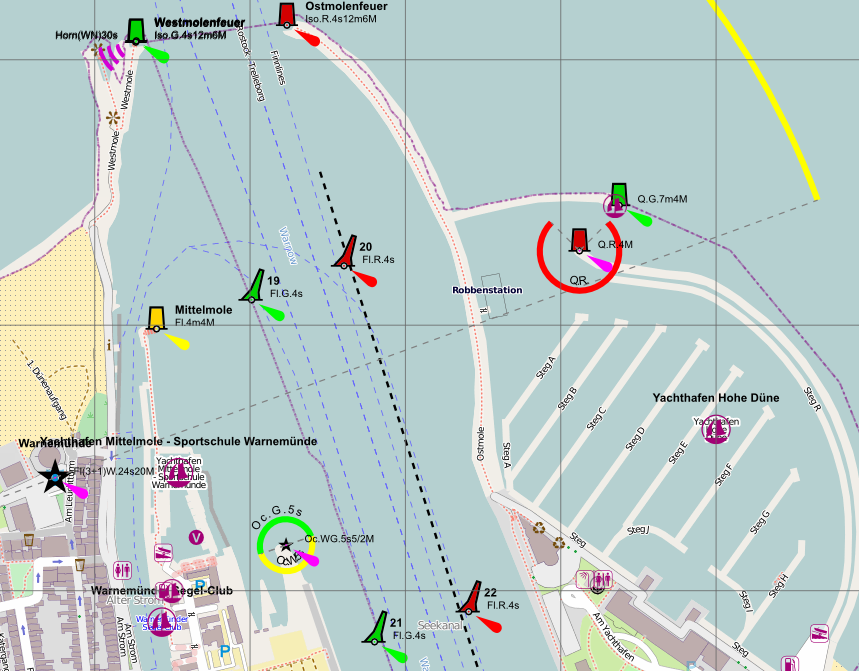
\includegraphics[width=10cm]{style-seamap.png}

\end{frame}

\hypersetup{urlcolor=cyan}
\begin{frame}{Lokalisierte Karten :\hfill\href{http://toolserver.org/~osm/locale/ru.html}{toolserver.org/~osm/locale/ru.html}}
	\begin{center}
		\vspace{-1cm}
		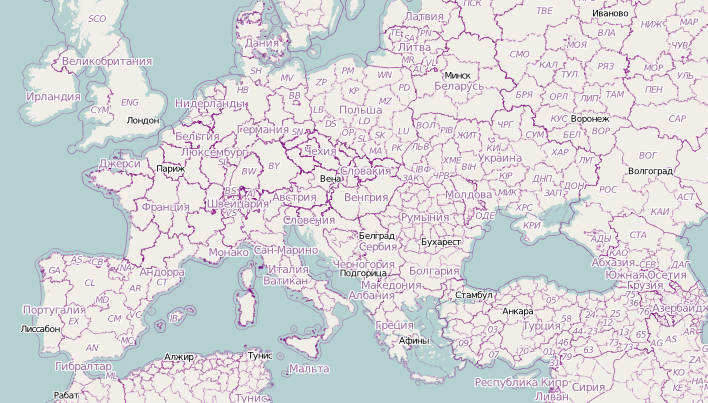
\includegraphics[height=6.5cm]{style-russ.png}
	\end{center}
\end{frame}
\hypersetup{urlcolor=blue}

%\begin{frame}{}

%\end{frame}

\begin{frame}{POI-Karten: z.B. OpenGastroMap}

 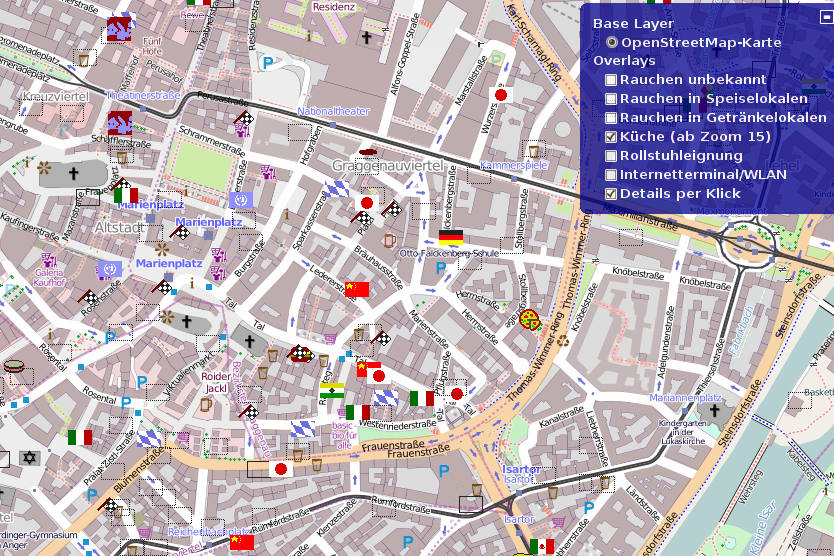
\includegraphics[width=10cm]{opengastromap-de.png}

\end{frame}

\begin{frame}{POIs Suchen: Overpass-Turbo.eu}

	Mittels Wizard: "`Museum in Bonn"'
\vfill
 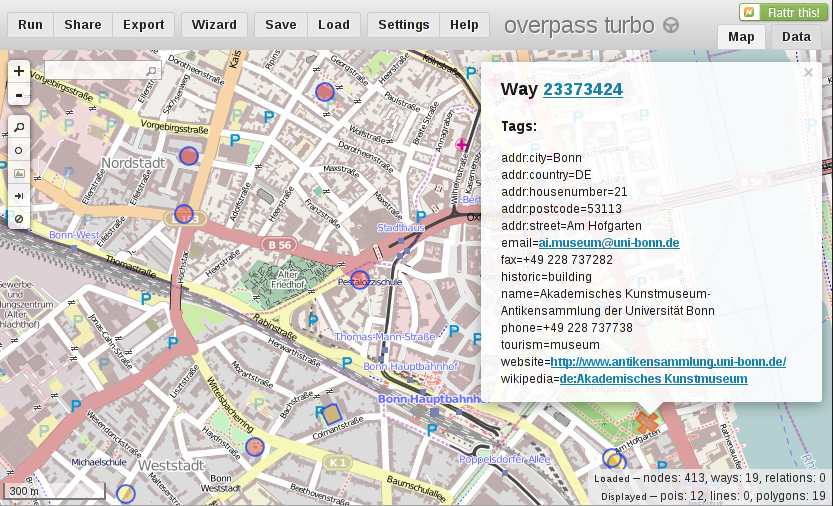
\includegraphics[width=10cm]{overpass.png}

\end{frame}

% OSM-Datenmodell

\section{OSM-Datenmodell}

\begin{frame}{Datenmodell}
Wurde von Informatikern ohne Geo-Vorbelastung erstellt:
\begin{itemize}
  \item Basisobjekt: Punkt (Koordinaten), $\Rightarrow$ "`Node"' 
\includegraphics[width=0.5cm]{node.png}
  \begin{itemize}
    \item POIs
    \pause
    \item Teile von Wegen
  \end{itemize}
  \item Linienzüge sind eine Reihe von Nodes, $\Rightarrow$ "`Way"' 
\includegraphics[width=0.5cm]{way.png}
  \begin{itemize}
    \item Wege, Flüsse, Hecken etc.
    \item können geschlossen sein: Gebäude, Flächen
  \end{itemize}
  \pause
  \item Gruppierungen von Ways/Nodes $\Rightarrow$ "`Relations"' 
\includegraphics[width=0.5cm]{relation.png}
  \begin{itemize}
    \item Streckenrelationen, zB ÖPNV-Routen, Radrouten
    \item Multipolygone
    \item Abbiegebeschränkungen (Way:von, Way:nach, Node:über)
    \item Meta-Relationen, zB für Verkehrsverbünde
  \end{itemize}
\end{itemize}

\end{frame}

\subsection{Tagging}

\begin{frame}{Datenmodell: Tagging}

Jedes Element kann \emph{beliebige Anzahl} Eigenschaften "`Tags"' haben.

Sie legen den Typ und die Eigenschaften des Objektes fest:
\begin{itemize}
  \item POIs
  \item Wege (Strassen, Schienen, ...)
  \item Landnutzungen (Wälder, Wiesen, ...)
\end{itemize}

\pause

Ein "`Tag"' besteht aus Schlüssel und Wert, genannt "`key"' + "`value"'.

\pause

Der Key gibt die Objektgruppe an, der Value den Objekttyp.

 Paare sind Freitext -- z.B.:
\begin{itemize}
  \item amenity = cafe 
\includegraphics[width=0.5cm]{cafe.png}
  \item highway = footway 
\includegraphics[width=1cm]{footway.png}
  \item building = yes  
\includegraphics[width=0.5cm]{building.png}
\end{itemize}

\end{frame}


\section{Mitmachen!}

% Wie bei OSM mitmachen?
% * Account anlegen auf osm.org
% * learnosm.org
% * Tab 'Edit'

\begin{frame}{Mitmachen!}
\begin{itemize}
  \item Account anlegen auf osm.org
	\begin{itemize}
		\item Kein Realname, keine Einladung n"otig - nur E-Mail und Passwort.
	\end{itemize}
  \item Tab "`Edit"' auf osm.org
	\begin{itemize}
		\item Kein Freischalten, keine "`Reputation"' n"otig - Alle "Anderungen sofort live!
	\end{itemize}
  \item Tutorial:  \href{http://learnosm.org/}{learnosm.org} 
  \item Dokumentation: \href{http://wiki.openstreetmap.org}{wiki.openstreetmap.org}
  \item Immer noch etwas unklar? $\Rightarrow$ Mailingliste \href{http://lists.openstreetmap.org/listinfo/talk-de}{talk-de}
  \item Weltweite \href{http://usergroups.openstreetmap.de/}{Stammtische}
\end{itemize}

\end{frame}


\section{Ende}

\begin{frame}{Vielen Dank für die Aufmerksamkeit!}

  Folien zur OpenStreetMap-Einführung am 8.4.2014, BRG Kepler
\vspace{1cm}

Folien unter: 
\includegraphics[width=1cm]{cc-by-sa.pdf}.
\vspace{1cm}

Erstellt mittels \LaTeX Beamer, Quelltext: \href{https://github.com/species/vortrag-osm-kepler}{Github}.
\vspace{1cm}

\href{mailto:michael.maier@student.tugraz.at}{Michael Maier}

Twitter: \href{https://twitter.com/osmgraz}{@osmgraz}
\end{frame}

\begin{frame}{Aufgaben}

  Folgende Webseiten erkunden:

  \begin{itemize}
    \item Hauptseite: osm.org
    \item Fahrradrouting: www.finnder.com
    \item maps.stamen.com/watercolor/
    \item openpistemap.org
    \item openptmap.org
    \item overpass-turbo.eu
  \end{itemize}

\end{frame}


\end{document}
